\mychapter{The board}
\label{ch:board}
\section{Creating a board}
Find something round to use as a template for the board spaces, then find a
scrap piece of paper to draw the board on. If you are using a pair of $N$-sided
dice, then the paper should have height of at least $N \times 1.5 \times D$ and
a width of at least $N \times D$, where $D$ is the diameter of the round thing.

Put the round thing in the top corner, leaving a little space to all sides
for numbers and doodles. Draw a circle around it, then move it along so that
the round thing touches the circle you just drew and draw another. Next,
move the round thing down so that it just touches the two circles and draw your
third circle. This way, the new circle will have the support of two previous
circles, which helps keeping them aligned. Keep going until you have $N \times
N$ circles. Don't worry if they don't match up perfectly.

Starting from the top corner, put the numbers $1$ through $N$ next to the
circles along both edges going from the corner. This is to help you find the
right spaces when playing.

To help remind you which parts are up- and down-stream respectively, consider
drawing some waves around the down-stream part of the board and some mountains
around the up-stream part. If you need inspiration for drawing mountains, look
up the cartographer Erwin Raisz.


\section{Example board}
\label{sec:example_board}
The following is an example board for a pair of six-sided dice.
\begin{center}
    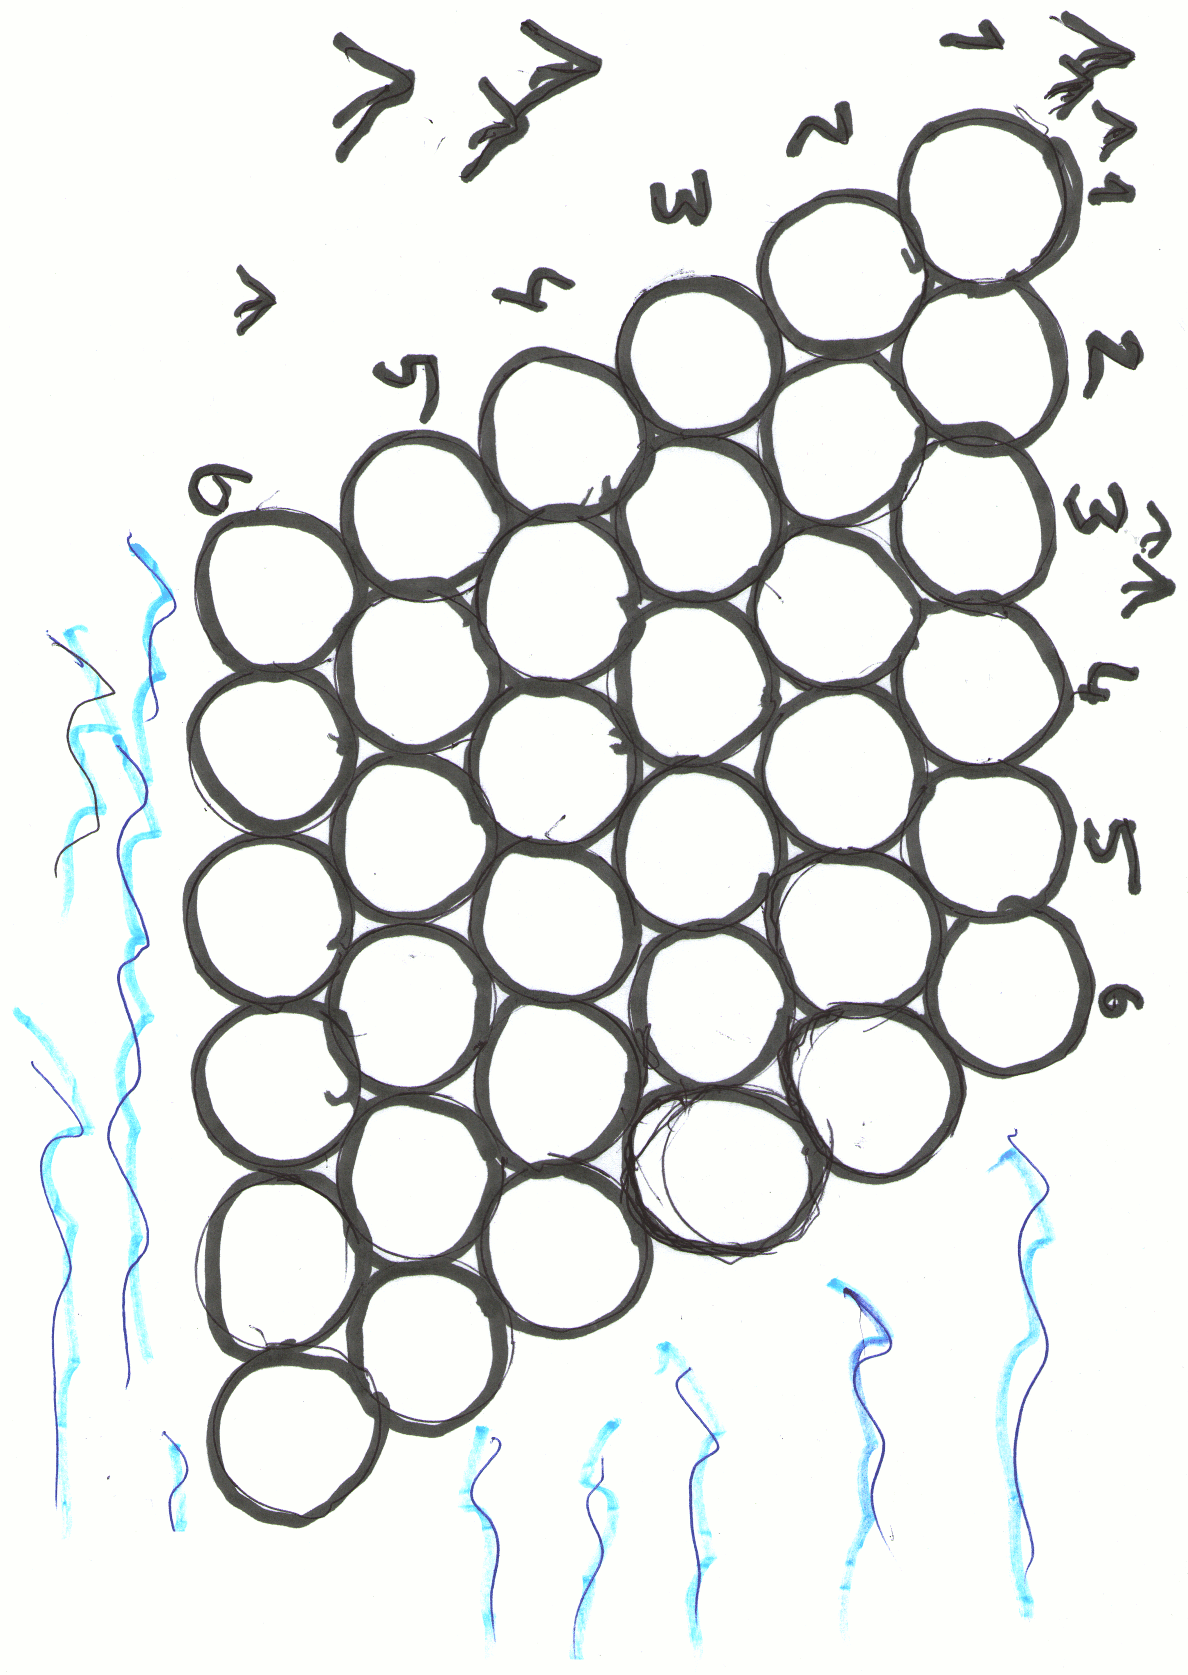
\includegraphics[width=0.84\textwidth]{board}
\end{center}
